\chapter{Related Work }
\label{sec:related_work}

This chapter gives a brief overview of available planning methods. One distinguish between roadmap, cell decomposition, potential field, sampling-based and graph-search planning methods\footnote{A similiar classification can be found in the bachelor thesis Robotic Arm Motion Planning by Markus Br\"andle}. A detailed description can be found in (Siegwart, 2004, \cite{Siegwart2004}), (Karaman, 2011, \cite{Karaman2011}) and (Bertsekas, 1995, \cite{Bertsekas1995}).

\section{Roadmap Path Planning}

This method is based on constructing a graph network consisting of lines in the obstacle-free configuration space\footnote{Vector space defined by the generalized coordinates of a system.}. The actual planning is then reduced to connecting the initial and goal state of the robot to the network and searching for feasible paths between them. In the following, two roadmap approaches are described.

\subsection{Visibility Graph}

The visibility graph is mostly suitable and highly efficient for sparse 2D configuration spaces with polygonal obstacles. The nodes of the graph include the vertices of the obstacles as well as the initial and final point. Straight-line segments connect every nodes that are visible from each other (i.e. sight is not blocked by an obstacle), which also includes the edges of the polygons. Thus, the optimal path in terms of length between start and goal state can be found (see Figure \ref{pics:visibility_graph}). The implementation of the visibility graph is straight forward, however, there are two major drawbacks of this method. First, the computational effort increases with the number of obstacles, which lowers the efficiency of the algorithm in dense environments. Second, the algorithm tends to generate a path as close as possible to nearby obstacles. However, the latter can be solved by expanding the size of the obstacles or using another roadmap method called the Voronoi diagram. 

\begin{figure} [h]
	\centering
	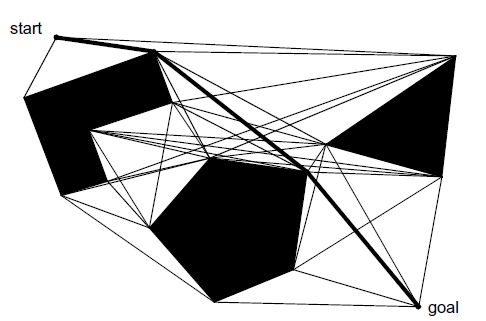
\includegraphics[width=0.5\textwidth]{images/visibility_graph.png}
	\caption{Visibility graph, 'this image is taken from \cite{Siegwart2004}'.}
	\label{pics:visibility_graph}
\end{figure}

\subsection{Voronoi Diagram}

In contrast with the visibility graph method, a Voronoi diagram (see Figure \ref{pics:voronoi_graph}) maximizes the distances between the robot and the obstacles in the configuration space (including the boundaries). It consists of equipotential line-segments constructed from points that are equidistant from two or more obstacles. 

\begin{figure} [h]
	\centering
	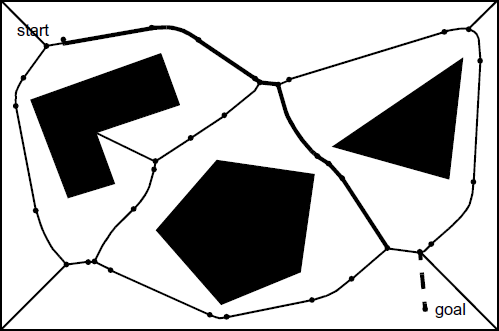
\includegraphics[width=0.5\textwidth]{images/voronoi_graph.png}
	\caption{Voronoi diagram, 'this image is taken from \cite{Siegwart2004}'.}
	\label{pics:voronoi_graph}
\end{figure}

\section{Cell Decomposition Path Planning}

The general idea of the cell decomposition method can be summarized as follows:

\begin{itemize}
	\item
	splitting of the configuration space into smaller non-overlapping regions called \textit{cells},
	\item
	constructing a \textit{connectivity graph} according to the cell-conjunctions,
	\item
	searching for a sequence in the connectivity graph that joins the initial with the goal cell,
	\item
	computation of a path passing through each cell of the sequence.
	
\end{itemize}

Depending on the cell division, one distinguish between exact and approximate cell decomposition.

\begin{itemize}
	\item
	Exact cell decomposition: Boundaries of the cells corresponds to the structure of the environment (see Figure \ref{pics:cell_decomposition}).
	\item
	Approximate cell decomposition: Division into cells results in an approximation of the map. 
\end{itemize}

\begin{figure} [h]
	\centering
	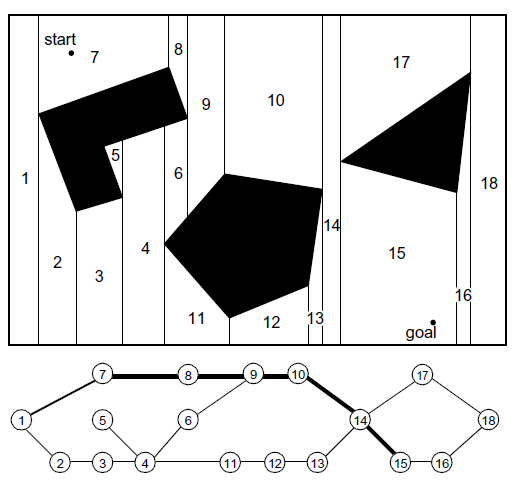
\includegraphics[width=0.7\textwidth]{images/cell_decomposition.png}
	\caption{Exact cell decomposition, 'this image is taken from \cite{Siegwart2004}'.}
	\label{pics:cell_decomposition}
\end{figure}

\section{Potential Field Path Planning}

The idea behind this method is to set up a gradient across the map, such that the robot, represented by a point, is attracted toward the goal, while being repulsed by the obstacles. As one can see in Figure \ref{pics:potential_field}, the resulting field (d) is thus the sum of a attractive (b) and a repulsive potential field (c). This method guides the robot smoothly towards its goal position while avoiding collision with obstacles (e). Potential field path planning can be used in high-dimensional configuration spaces. However, one major drawback of potential fields is the formation of local minima, in where the robot gets trapped. 

\begin{figure} [h]
	\centering
	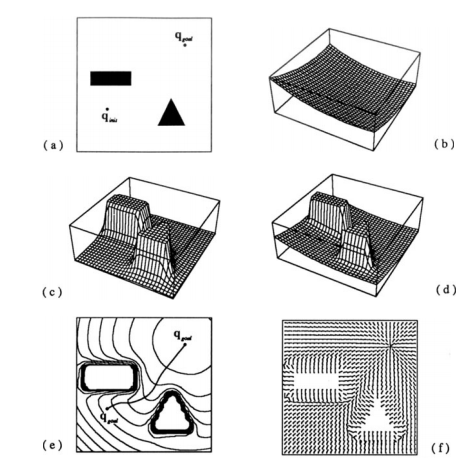
\includegraphics[width=0.9\textwidth]{images/potential_field.png}
	\caption{Different potential fields, 'this image is taken from \cite{Latombe2012}'.}
	\label{pics:potential_field}
\end{figure}

\section{Sampling-Based Algorithms for Path Planning}

These methods are using some form of sampling-based algorithm to produces potential configurations, which are subsequently checked on their feasibility by a collision detector. They can be easily adapted to high-dimensional configuration spaces. One distinguish between multi- and single-query methods. 

\begin{itemize}
	\item
	Multi-query methods are mostly suitable for static environments and consists of a preprocessing phase, where a roadmap is constructed, and a query phase, where a path is planned to connect the start and goal configuration. 
	\item
	In single-query methods, the robot constructs the roadmap while simultaneously searching for a path between initial and goal configuration. Since these methods works online, they are capable for usage in dynamic environments.
\end{itemize}


\subsection{Rapidly-Exploring Random Tree}

RRT (see Figure \ref{pics:rrt}) is a single-query path planning algorithm. It builds a tree of possible configurations that expands from the initial state and tends to cover the whole obstacle-free workspace. At each iteration, a new random node is sampled and the necessary measures are taken to connect it feasible to the tree. A modified version of this algorithm is used for the path planner of this bachelor thesis.

\begin{figure} [h]
	\centering
	\includegraphics[width=0.7\textwidth]{images/rrt.png}
	\caption{RRT tree after (a) 250, (b) 500, (c) 2500 and (d) 10'000 iterations, 'this image is taken from \cite{Karaman2011}'.}
	\label{pics:rrt}
\end{figure} 

\subsection{Probabilistic Roadmap}

Probabilistic roadmap (PRM) (see Figure \ref{pics:prm}) is a multi-query path planning method. In a first step, random samples from the configuration space of the robot are taken. Second, these samples are being checked whether they are located in the free space. In case of being in the obstacle free space, a local planner attempts to connect them to other existing nearby configurations. After the initial and goal states are connected to the constructed roadmap, a graph search algorithm (see also Section ~\ref{sec:graph_search})  is applied to determine a path between both nodes.  

\begin{figure} [h]
	\centering
	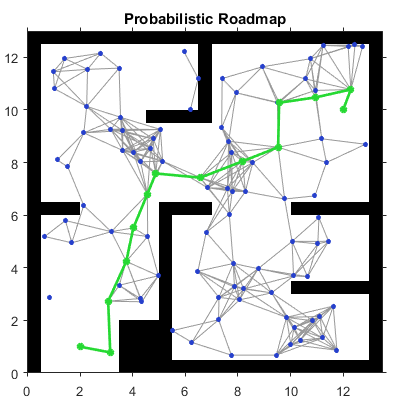
\includegraphics[width=0.7\textwidth]{images/prm.png}
	\caption{An example of a probabilistic roadmap with the path from an initial to a goal configuration marked in green, 'this image is taken from \textit{Mathworks} under the topic Probabilistic Roadmaps'.}
	\label{pics:prm}
\end{figure} 

\section{Graph-Search Algorithms}
\label{sec:graph_search}
This section gives a brief overview of the most common common graph-search algorithms.
\subsection{Lin-Kernighan Heuristic}
The Lin-Kernighan heuristic is an algorithm which deletes existing connections between configurations and reconnects them in other possible ways to generate a more optimal solution. It is commonly used for tasks related to traveling salesman problem\footnote{Searching the shortest route through a list of states.}.

\subsection{Greedy Algorithm}
The Greedy algorithm makes the locally optimal choice at each node. In general, this method does not generate a global optimal sequence of configurations.

\subsection{Label Correcting Algorithm}

With the label correcting algorithm (LCA), the shortest path in a graph network between an initial and a terminal node can be found, assuming the transition cost $a_{ij}$ between state i and j is positive. The algorithm can be summarized in 4 steps (detailed description of the variables and the steps can be found in \cite{Bertsekas1995}): 

\begin{enumerate}
	\item Place the initial node $S$ in the OPEN BIN and set: $d_S=0$ and $d_j=\infty$ $\forall j$ ($d_q$: cost to move from state $S$ to state $q$)
	\item Remove a node $i$ from the OPEN BIN and execute step 3 for all children $j$ of $i$.
	\item If $d_i + a_{ij} < min(d_j, d_T)$ ($d_ {T}$ is the final node), set $d_j = d_i + a_{ij}$ and $i$ to be the parent of $j$. If $j \neq T$, place $j$ in the OPEN BIN if it is not already there. 
	\item If the OPEN BIN is empty, the algorithm is done, else go back to step 1. 
\end{enumerate}

There are multiple options in selecting a node to be removed from the OPEN BIN in step 2, which results in different algorithms:

\begin{itemize}
	\item Depth-first search: Last in, first out. 
	\item Best-first search: Remove best label first (Dijkstra's method). A generalization of this algorithm is A*. By adding a lower bound to the cost function, non-optimal nodes can be excluded.
	\item Breadth-first search: First in, first out (Bellman-Ford). 
\end{itemize}